\documentclass[tikz, border=10pt]{standalone}

\usepackage{tikz}
\usetikzlibrary{snakes}

% command to draw a pendulum
\newcommand{\physicalpendulum}{
    \pgfpathmoveto{\pgfpoint{0cm}{2cm}}
    \pgfpathcurveto{\pgfpoint{0.2cm}{2cm}}{\pgfpoint{0.2cm}{2cm}}{\pgfpoint{1cm}{1cm}}
    \pgfpathcurveto{\pgfpoint{1.75cm}{0cm}}{\pgfpoint{1.8cm}{0cm}}{\pgfpoint{2cm}{-2cm}}
    \pgfpathcurveto{\pgfpoint{2.2cm}{-4cm}}{\pgfpoint{2.3cm}{-4.2cm}}{\pgfpoint{2.5cm}{-5cm}}
    \pgfpathcurveto{\pgfpoint{2.7cm}{-5.8cm}}{\pgfpoint{3cm}{-6cm}}{\pgfpoint{3cm}{-7cm}}
    \pgfpathcurveto{\pgfpoint{3cm}{-8cm}}{\pgfpoint{2.25cm}{-8.75cm}}{\pgfpoint{2cm}{-9cm}}
    \pgfpathcurveto{\pgfpoint{1.75cm}{-9.25cm}}{\pgfpoint{1cm}{-10cm}}{\pgfpoint{0cm}{-10cm}}
    \pgfpathcurveto{\pgfpoint{-2cm}{-10cm}}{\pgfpoint{-3cm}{-8cm}}{\pgfpoint{-3cm}{-7cm}}
    \pgfpathcurveto{\pgfpoint{-3cm}{-3cm}}{\pgfpoint{-1cm}{-2cm}}{\pgfpoint{-1cm}{-1cm}}
    \pgfpathcurveto{\pgfpoint{-1cm}{0cm}}{\pgfpoint{-.5cm}{2cm}}{\pgfpoint{0cm}{2cm}}
    \pgfusepath{stroke, fill}
}

\begin{document}
    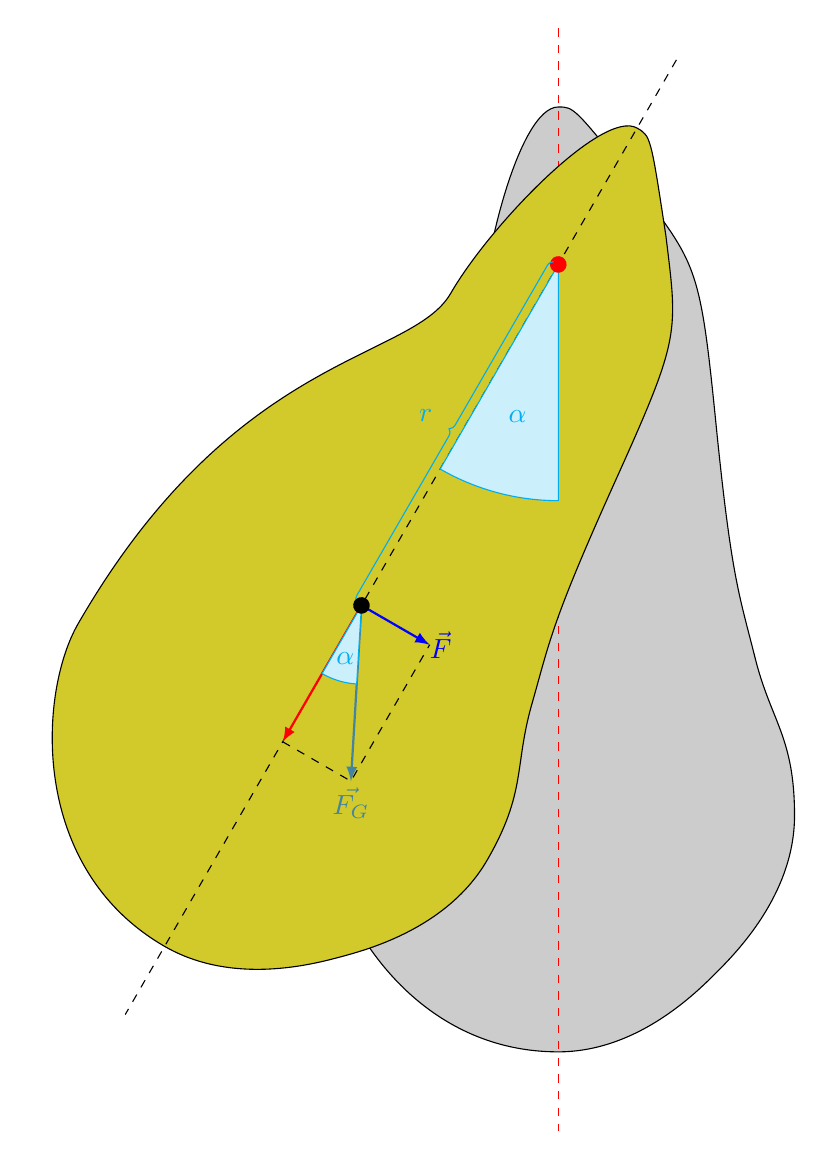
\begin{tikzpicture}
        % draw first pendulum
        % set pendulum's color
        \pgfsetfillcolor{black!20!white}
        \physicalpendulum
        % draw axis of symmetry of first pendulum
        \draw[color=red, dashed] (0, 3) -- (0, -11);
        % rotate coordinate system
        \pgftransformrotate{-30}
        % set pendulum's color
        \pgfsetfillcolor{yellow!80!black}
        % draw second pendulum
        \physicalpendulum
        % second pendulum's axis of symmetry
        \draw[dashed] (0, 3) -- (0, -11);
        \pgftransformrotate{30}
        % draw angle between pendulums
        \filldraw[fill=cyan!20, draw=cyan] (0, 0) -- ++(0, -3) arc (-90:-120:3) -- cycle;
        \node[cyan] at (-105:2) {$\alpha$};
        \pgftransformrotate{-30}
        % draw hanging point of pendulums
        \fill[color=red] (0, 0) circle (3pt);
        % draw distance from hanging point to second pendulum's center of mass
        \draw[snake=brace, mirror snake, raise snake=2pt, color=cyan] (0, 0) -- +(0, -5);
        \node[color=cyan] at (-0.5, -2.5) {$r$};
        % draw all force affect to pendulum
        \draw[-latex, thick, color=red] (0, -5) -- +(0, -2);
        \draw[-latex, thick, color=blue] (0, -5) -- +(1, 0) node[xshift=4pt] {$\vec{F}$};
        \draw[-latex, thick, color=cyan!60!black] (0, -5) -- (0, -7 -| 1, -5) node[yshift=-8pt] {$\vec{F_G}$};
        \draw[dashed] (0, -7) -- (1, -7) -- (1, -5);
        \filldraw[fill=cyan!20, draw=cyan] (0, -5) -- +(-63.5:1) arc (-63.5:-90:1) -- cycle;
        \draw[color=cyan] (0, -5) +(-77:0.7) node {$\alpha$}; 
        \fill[color=black] (0, -5) circle (3pt);
    \end{tikzpicture}
\end{document}